\documentclass[12pt]{spieman}  % 12pt font required by SPIE;
%\documentclass[a4paper,12pt]{spieman}  % use this instead for A4 paper
\usepackage{amsmath,amsfonts,amssymb}
\usepackage{graphicx}
\usepackage{setspace}
\usepackage{tocloft}

\title{Age Estimation; Morphs; Facial Recognition}

\author[a]{Krivonosova Ekaterina and Chernikova Polina}
\affil[a]{Samara University}

\renewcommand{\cftdotsep}{\cftnodots}
\cftpagenumbersoff{figure}
\cftpagenumbersoff{table} 
\begin{document} 
\maketitle

\begin{spacing}{2}   % use double spacing for rest of manuscript

\section{An Ensemble CNN2ELM for Age Estimation}
\label{sect:intro}  % \label{} allows reference to this section
Therefore, age estimation should not only consider race and gender as factors but also yield a novel structure in which differentiable features can be extracted. CNN2ELM includes three convolutional neural network  structures and two extrame learning machine (ELM) structures. Our proposed networks are pretrained on the ImageNet dataset and then fine-tuned on the IMDB-WIKI dataset [22] before being fine-tuned on MORPH-II, Adience benchmark, and ChaLearn Looking at People 2016 (LAP-2016) datasets. During the validation and test stages, the three networks are used to extract features from the same image, and a discriminative and robust feature set is achieved by fusing these features. Based on the fusion features, ELM classifies these features into one of the age groups. It not only sufficiently exploits the CNN but also utilizes the outstanding classification and regression properties of the ELM. The major contributions of this paper are as follows: 

%Список маркированный
\begin{itemize}
  \item {We propose an ensemble CNN2ELM approach for performing age estimation. The structure combines the CNN with the ELM to perform age estimation in a hierarchical fashion, in which the CNN is used to extract features, while the ELM predicts age based on the image of a person age.}
  \item The highlights of our CNN2ELM structure are feature enhancement and age grouping. Our system comprises three CNNs and two ELMs (i.e., Race-Net + AgeNet + Gender-Net + ELM classifier + ELM regressor (RAGN)”). Table~\ref{tab:fonts}
  \item Finally, we present the process of integrating the synergyof the hybrid structure in detail, including the design of the layers in the CNN. By a comprehensively considering the factors mentioned above and after many experiments, we set the size of the input feature map as 227 × 227, which is showed in Fig.~\ref{fig:example1}
\end{itemize}

\begin{table}[ht]
\caption{The data set selected from MORPH-II for our experiment.} 
\label{tab:fonts}
\begin{center}       
\begin{tabular}{|l|l|l|l|} %% this creates four columns
%% |l|l| to left justify each column entry
%% |c|c| to center each column entry
%% use of \rule[]{}{} below opens up each row
\hline
\rule[-1ex]{0pt}{3.5ex}   & Female & Male & Female and Male\\
\hline\hline
\rule[-1ex]{0pt}{3.5ex} Black & 5,757 & 36,809 & 42,560  \\
\hline
\rule[-1ex]{0pt}{3.5ex}  White & 2,601 & 7,999 & 10,600   \\
\hline
\rule[-1ex]{0pt}{3.5ex} Black and White & 8,358 & 44,802 & 53,160  \\
\hline
\end{tabular}
\end{center}
\end{table} 

\begin{figure}
\begin{center}
\begin{tabular}{c}
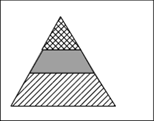
\includegraphics[height=5.5cm]{1.jpg}
\end{tabular}
\end{center}
\caption 
{ \label{fig:example1}
Full schematic diagram of our network architecture. } 
\end{figure} 


\section{RELATED WORK}

\subsection{Hybrid Neural Network }
\label{sect:title}
System CNN has been successfully applied to various fields, and image recognition, in particular, is a hot area of research. The approach reduces the number of parameters in the network and reduces the training time. Based on the above results, we decided to integrate CNN with other classifiers to improve the classification accuracy. 

\subsection{Fusion Methods}
Fusion is a popular technology in biometrics, and it is most commonly used to fuse decisions or features in a hierarchical learning system. One of the most successful examples is the ensemble system [20]. This system proves that several classifiers with similar training characteristics have different generalization performances, and fusing these classifiers may or may not lead to a better performance than that of the best classifier in this ensemble system while reducing the global risk of making a poor decision. 

\subsection{Age Grouping }
In recent years, facial age grouping has been widely used for age estimation and many methods have been proposed. Kwon and da Vitoria Lobo [5] first introduced the age grouping method for age estimation, which starts by categorizing images into three age groups: infants, youth, and seniors. During the experiments, 47 images were used to verify the performance of the proposed method.
For Gender-Net, the selected dataset and settings of the network and parameters are the same as for Race-Net. Figure~\ref{fig:example2} shows the process of Gender-Net.

\begin{figure}
\begin{center}
\begin{tabular}{c}
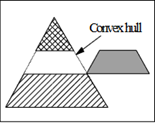
\includegraphics[height=5.5cm]{2.jpg}
\end{tabular}
\end{center}
\caption 
{ \label{fig:example2}
The process of Race-Net. The color indicates the output of convolutional layers. } 
\end{figure} 

Next, the outputs of the convolutions add an additive bias and an element-wise nonlinear activation function is then applied to the front results. We have Equation~(\ref{eq:fov})

\begin{equation}
\label{eq:fov}
\eta_{ij}^{mn} = \sigma{(b_{ij}+\sum\nolimits_{\delta}\sum\nolimits_{p=0}^{P_{i}-1}\sum\nolimits_{q=0}^{Q_{i}-1}}\omega_{ij}^{pq})\,
\end{equation}
where $b_{ij}$ represents the bias of this feature map, and $\sigma$ indexes over the set of the feature maps in the $(i - 1)th$ layer, which are connected to this convolutional layer. $\omega_{ij\sigma}^{pq}$ denotes the value at the position ( p, q) of the kernel, which is connected to the kth feature map.

\section{PRELIMINARY INFORMATION}
\label{sect:sections}
The purpose of our feature vector fusion is to obtain an enhanced feature vector that is beneficial to the ELM classifiers. Figure~\ref{fig:example3} shows the process of feature fusion. Because classifiers learn more correlative and useful information, they can achieve a better generalization performance.
The Design of Our Ensemble Structure:

\begin{figure}
\begin{center}
\begin{tabular}{c}
\includegraphics[height=5.5cm]{3.jpg}
\end{tabular}
\end{center}
\caption 
{ \label{fig:example3}
The process of feature fusion. During the validation and test stage, Race-Net, Age-Net, and Gender-Net are used to extract features from the same image. } 
\end{figure} 

\begin{enumerate}
\item Convolutional Layer;
\item Contrast Normalization Layer;
\item Max Pooling Layer.
\end{enumerate}

To achieve the target, two normalization operations, i.e., subtractive and divisive, are performed. ηmnk denotes the value of an unit at position $(m, n)$ in the kth feature map. We have Equation~(\ref{eq:fov2})

\begin{equation}
\label{eq:fov2}
\zeta_{mnk}= \eta_{mnk}-\sum\nolimits_{p=-\frac{P_{i}-1}{2}}^{\frac{P_{i}-1}{2}}\sum\nolimits_{p=-\frac{Q_{i}-1}{2}}^{\frac{Q_{i}-1}{2}}\sum\nolimits_{j=1}^{J_{j}}\omega\,
\end{equation}
where $\eta_{mnk}$ is a normalized Gaussian filter with the size of 7 × 7 at the first stage and 5 × 5 at the second stage. $z_{mnk}$ not only represents the input of the divisive normalization operations but also denotes the output of the subtractive normalization operations. Equation~(\ref{eq:fov3}) expresses the operator of the divisive normalization: 

\begin{equation}
\label{eq:fov3}
\eta_{mnk}=\frac{z_{mnk}}{(max(M,M(m,n)))}\,
\end{equation}


\end{spacing}
\end{document}